%==============================================================
%  The Longest-Answer Heuristic:
%  Characterizing and Mitigating Answer-Length Bias in
%  LLM-Generated Multiple-Choice Questions
%==============================================================
\documentclass[10pt,twocolumn]{article}

% ---- packages ----
\usepackage[T1]{fontenc}
\usepackage[utf8]{inputenc}
\usepackage[protrusion=true,expansion=false]{microtype}
\usepackage[margin=0.78in]{geometry}
\usepackage{amsmath,amssymb}
\usepackage{graphicx}
\usepackage{booktabs}
\usepackage{caption}
\usepackage{subcaption}
\usepackage{xcolor}
\usepackage[ruled,vlined,linesnumbered]{algorithm2e}
\usepackage[numbers,sort&compress]{natbib}
\usepackage{enumitem}
\usepackage{balance}
\usepackage[hidelinks,breaklinks]{hyperref}
\usepackage{url}

\definecolor{accent}{RGB}{44,74,126}
\captionsetup{font=small,labelfont=bf}
\graphicspath{{../figures/}}

\setlength{\columnsep}{0.28in}
\hyphenation{multi-ple ex-ploit-abil-ity con-struct-ir-rel-e-vant}

% ---- title ----
\title{\vspace{-1.4em}\bfseries The Longest-Answer Heuristic:\\
Characterizing and Mitigating Answer-Length Bias in\\
LLM-Generated Multiple-Choice Questions as a\\
Threat to Assessment Integrity}

\author{%
Steven\thanks{Department of Artificial Intelligence, Kyungdong University
Global Campus, Chuncheon, Republic of Korea. Correspondence:
\texttt{author@kduglobal.ac.kr}.}\\
\small Department of Artificial Intelligence\\
\small Kyungdong University Global Campus
}
\date{}

%==============================================================
\begin{document}
\maketitle

\begin{abstract}
\noindent
Large language models (LLMs) are increasingly used by educators and students
to author multiple-choice questions (MCQs) at scale. We investigate a
specific and underexamined failure mode: a systematic correlation between the
\emph{length} of an answer option and its probability of being keyed correct.
When present, this correlation reintroduces a classical item-writing flaw---
``the longest option is correct''---at machine scale, furnishing test-takers
with a construct-irrelevant ``pick-the-longest'' heuristic that inflates
scores without measuring knowledge. We make four contributions. First, we
formalize \emph{answer-length leakage} and define a reusable, model-agnostic
measurement suite: Longest-Answer Accuracy (LAA), an \emph{Exploitability}
index $E$ that normalizes a guessing strategy's advantage over chance, a
verbosity differential $\bar\delta$, and a length-only leakage AUC. Second, we
release an open, provider-agnostic data-collection harness \emph{designed to
elicit} MCQs from six widely used assistants under an identical, length-neutral
prompt, so that the bias can be \emph{measured}---rather than assumed---once the
harness is run with sanctioned API access (a step not performed in this version). Third, we contribute
a generation-time mitigation toolkit---an auditing gate, a length-balanced
rewrite planner, length-matched adversarial distractors, and form-level
key-length balancing---with a measured before/after protocol. Fourth, we
provide a fully reproducible analysis pipeline. Because we did not have
sanctioned API access to all six commercial systems at submission time, the
quantitative results reported here are generated from a clearly labeled
\emph{synthetic} corpus that exercises the entire pipeline end to end; on that
corpus the toolkit reduces exploitability from $E{=}{+}0.36$ to near parity
($E{=}{-}0.06$) and cuts leaky items from $71\%$ to $3\%$. We position the
measurement suite and mitigations as deployable safeguards and provide a
preregistered protocol for the real-model and human-subject studies needed to
confirm the effect in the wild.
\end{abstract}

\vspace{0.4em}
{\small\noindent\textbf{Keywords:} large language models; multiple-choice
questions; automatic question generation; assessment validity; item-writing
flaws; construct-irrelevant variance; test-wiseness; verbosity bias;
educational integrity; mitigation.}
\vspace{0.6em}

%==============================================================
\section{Introduction}
\label{sec:intro}

Automatic question generation (AQG) with large language models (LLMs) has
moved from research prototype to everyday classroom tool. Instructors use
chat assistants to draft quizzes in seconds; students use the same assistants
to generate practice items; publishers and learning platforms embed them in
content pipelines. The appeal is obvious---authoring high-quality
multiple-choice questions (MCQs) by hand is slow and expensive
\citep{kurdi2020systematic}. But a question that is cheap to produce is not
necessarily \emph{valid}. An MCQ is valid only insofar as a correct response
reflects the intended knowledge or skill and nothing else. When a surface
feature of the item---unrelated to its content---predicts the keyed answer,
the item leaks. Test-takers who learn to read that feature can score above
chance without knowing the material, and the score loses its meaning
\citep{messick1989validity}.

This paper concerns one such surface feature: \textbf{the length of the answer
options}. A long-standing rule of professional item writing is that the
correct option should not be conspicuously longer than the distractors,
precisely because writers tend---often unconsciously---to over-qualify the key
with hedges, conditions, and exceptions, making it both longer and more
``textbook-correct'' in appearance
\citep{haladyna2002review,tarrant2006frequency}. Skilled test-takers exploit
this: choosing the longest option is a documented component of
\emph{test-wiseness}, the ability to use cues in an item's form rather than its
content \citep{millman1965testwiseness}. The concern we raise is that LLMs,
trained on enormous corpora of human-written text and optimized with human
feedback that can reward thoroughness and verbosity
\citep{zheng2023judging,saito2023verbosity}, may reproduce or even amplify
this tendency---generating keys that are systematically longer than the
distractors they sit beside. If so, every quiz produced this way ships with a
built-in cheat code, and the more an institution leans on LLM-authored
assessment, the more pervasive the leak becomes.

\paragraph{Why this matters now.} Three trends compound the risk.
(i)~\emph{Scale}: a single prompt can yield hundreds of items, so a small
per-item bias becomes a large aggregate exposure.
(ii)~\emph{Automation bias}: users tend to trust machine-generated artifacts
and review them less critically, so flawed items are less likely to be caught
in editing \citep{frontiers2026automation}.
(iii)~\emph{Homogeneity}: when many instructors use the same few models, the
same exploitable pattern recurs across courses and institutions, making the
heuristic easy for students to learn and transfer. A bias that an individual
human writer might exhibit idiosyncratically becomes, under LLMs, a systematic
and \emph{predictable} property of the tool.

\paragraph{Objectives.} We set out to (1) make the phenomenon
\emph{measurable} with precise, reusable metrics; (2) make it
\emph{collectable} with an auditable, provider-agnostic harness that \emph{can
elicit} items under a length-neutral prompt; (3) make it \emph{fixable} at generation
time with lightweight, deployable mitigations; and (4) make the whole pipeline
\emph{reproducible}. We deliberately treat the prevalence of the bias as an
empirical question to be answered by measurement, not as a settled fact.

\paragraph{Research questions.}
\begin{description}[leftmargin=1.4em,itemsep=1pt,topsep=2pt]
\item[RQ1.] Can answer-length leakage in LLM-generated MCQs be defined and
quantified with a model-agnostic, exploitability-oriented metric suite?
\item[RQ2.] How large is the leakage, and does it vary by model, subject, and
difficulty?
\item[RQ3.] Does a ``pick-the-longest'' strategy yield an above-chance score,
and how much information does length alone carry about the key?
\item[RQ4.] Can generation-time mitigations remove the length signal---measured
before/after on the option-length metrics above---and by how much? (We evaluate
\emph{option-length characteristics}, not pedagogical item quality; assessing
quality remains future work, \S\ref{sec:future}.)
\end{description}

\paragraph{Contributions and scope.} Our contributions are the metric suite
(\S\ref{sec:metrics}), the collection harness (\S\ref{sec:harness}), the
mitigation toolkit (\S\ref{sec:mitigation}), and the reproducible analysis
(\S\ref{sec:results}). \textbf{An explicit caveat governs the whole paper:}
the numbers reported in \S\ref{sec:results} are produced from a
\emph{synthetic} corpus with injected, known bias levels. They exist to
verify that the metrics behave correctly and that the mitigations work; they
are \emph{not} measurements of any real commercial model and must not be read
as such. \S\ref{sec:limitations} states this plainly and
\S\ref{sec:future} gives the preregistered protocol for the real-model and
human-subject studies required to estimate the effect in deployment.

%==============================================================
\section{Related Work}
\label{sec:related}

\subsection{Item-writing flaws and assessment validity}
The psychometric literature has catalogued item-writing flaws for decades.
\citet{haladyna1989taxonomy} introduced a taxonomy of item-writing rules,
refined into an evidence-based guideline set by \citet{haladyna2002review};
among the rules is the explicit injunction that the correct option should not
be made longer than the distractors. \citet{tarrant2006frequency} found such
flaws to be common in real examinations and showed they disproportionately
affect high-achieving and borderline candidates. \citet{downing2005effects}
demonstrated that flawed items change pass/fail outcomes for a non-trivial
fraction of examinees, establishing that these are consequential, not cosmetic,
defects. \citet{rodriguez2005three} provides meta-analytic evidence on option
counts. Underlying all of this is \citeauthor{messick1989validity}'s framework
of \emph{construct-irrelevant variance}: score variance attributable to
features other than the target construct \citep{messick1989validity}. A
length cue is a textbook source of such variance, and the ability to use it is
the classical notion of \emph{test-wiseness}
\citep{millman1965testwiseness}. Our work imports these constructs into the
LLM setting and operationalizes ``the longest option is correct'' as a
measurable, exploitable quantity.

\subsection{Automatic question generation}
Surveys of AQG document rapid progress and persistent quality-control gaps
\citep{kurdi2020systematic}, with distractor generation a particular
challenge \citep{awalurahman2024distractor,qiu2020automatic}. The dominant
evaluation lens is fluency and answerability; the \emph{statistical validity}
of the generated key relative to its distractors---whether the key is
distinguishable by a surface feature---has received far less attention. Recent
work has begun to flag that AI-assisted authoring can \emph{increase} the rate
of item-writing flaws through automation bias
\citep{frontiers2026automation,an2026orchestrating}, and comparative studies of LLM
MCQ generators are emerging \citep{comparativeMCQ2025,benchmarker2026}. We
contribute the missing measurement: a direct, cross-model quantification of
answer-length leakage as an exploitable cue.

\subsection{Biases in LLMs as judges and as answerers}
Two adjacent literatures motivate the hypothesis that LLMs would exhibit a
length asymmetry. First, when LLMs act as \emph{judges}, they display a
\emph{verbosity bias}, preferring longer responses independent of quality
\citep{zheng2023judging,saito2023verbosity}. Second, when LLMs act as MCQ
\emph{answerers}, they exhibit \emph{selection} and \emph{token bias}---
sensitivity to option ordering and to the surface form of option
identifiers---making them ``not robust'' selectors
\citep{zheng2024robust,wang2024lookatthetext}. Both lines concern how models
\emph{consume} options. The complementary and largely open question, which we
take up, is how models \emph{produce} options: when an LLM writes the key and
its distractors, does it imprint a length signature on the key? If verbosity is
rewarded in generation, the key---the option the model is most ``committed''
to justifying---is exactly where extra length would accrue.

\subsection{The gap}
Prior work establishes (a) that ``longest-correct'' is a real, consequential
item-writing flaw in human-authored tests; (b) that LLMs are verbose and
length-sensitive as judges and answerers; and (c) that AI authoring can raise
flaw rates. No prior work, to our knowledge, (i)~defines a reusable
\emph{exploitability} metric for answer-length leakage, (ii)~measures it
\emph{across} the major commercial assistants under a common protocol, and
(iii)~pairs the measurement with a \emph{generation-time} mitigation toolkit
evaluated before/after. This paper targets that gap, and is explicit about
which parts are delivered as \emph{verified} tooling versus which require
sanctioned data collection to estimate real-world magnitude.

%==============================================================
\section{Formalizing Answer-Length Leakage}
\label{sec:metrics}

\paragraph{Item model.} An MCQ item is a tuple
$x=(s,\mathcal{O},k)$ where $s$ is the stem, $\mathcal{O}=(o_1,\dots,o_m)$ is
an ordered list of $m$ options, and $k\in\{1,\dots,m\}$ is the index of the
keyed-correct option. Let $\ell(o)$ denote a length measure of option $o$; we
use character count by default and report word count as a robustness check.
Let the random ``chance'' baseline for a uniform guess be $1/m$.

\paragraph{Longest-Answer Accuracy (LAA).} For a corpus
$\mathcal{D}=\{x_i\}_{i=1}^{N}$, define the score a student would obtain by
always selecting the longest option (ties broken uniformly at random):
\begin{equation}
\mathrm{LAA}(\mathcal{D})=\frac{1}{N}\sum_{i=1}^{N}
\frac{\mathbb{1}\!\left[k_i\in \arg\max_{j}\ell(o_{ij})\right]}
{\bigl|\arg\max_{j}\ell(o_{ij})\bigr|}.
\label{eq:laa}
\end{equation}
$\mathrm{LAA}=1/m$ indicates no length signal; $\mathrm{LAA}>1/m$ indicates the
key tends to be the longest option.

\paragraph{Exploitability index $E$.} LAA is not comparable across items with
different option counts because the chance baseline $1/m$ differs. We normalize
the above-chance advantage to its maximum possible value:
\begin{equation}
E(\mathcal{D})=\frac{\mathrm{LAA}(\mathcal{D})-\bar{c}}{1-\bar{c}},
\qquad \bar{c}=\frac{1}{N}\sum_{i=1}^{N}\frac{1}{m_i},
\label{eq:expl}
\end{equation}
so $E=0$ when the strategy does no better than guessing and $E=1$ when the
longest option is \emph{always} the key. $E$ can be mildly negative if the key
is shorter than distractors on average. We adopt $E$ as our primary
cross-model, cross-subject comparison statistic because it answers the
practically meaningful question: \emph{how much of the way from chance to a
perfect cheat does length alone take you?}

\paragraph{Verbosity differential $\bar\delta$.} To capture magnitude in raw
units we define, per item, the gap between the key's length and the mean
distractor length, and average it:
\begin{equation}
\bar\delta(\mathcal{D})=\frac{1}{N}\sum_{i=1}^{N}\!\left(
\ell(o_{ik_i})-\frac{1}{m_i-1}\sum_{j\neq k_i}\ell(o_{ij})\right).
\label{eq:delta}
\end{equation}
We accompany $\bar\delta$ with a standardized effect size (the mean of the
per-item differential divided by its standard deviation) and a Wilcoxon
signed-rank test of $H_0:\bar\delta=0$.

\paragraph{Length-only leakage AUC.} Finally we ask how much a classifier that
sees \emph{only} option lengths can recover the key. For each item we form
$(m_i-1)$ key-vs-distractor pairs and score each option by $\ell$; the AUC is
the probability that a randomly chosen key outranks a randomly chosen
distractor by length:
\begin{equation}
\mathrm{AUC}=\Pr\!\left[\ell(o_{ik_i})>\ell(o_{ij})\right],\quad j\neq k_i.
\label{eq:auc}
\end{equation}
$\mathrm{AUC}=0.5$ is no leakage; $\mathrm{AUC}=1$ means length perfectly
ranks the key first. We complement the AUC with a logistic regression of the
binary ``is-key'' label on standardized option length, reporting the odds
ratio per one standard deviation of length, which expresses leakage as a
single interpretable multiplier. Crucially, the $m$ options of an item are
\emph{not} independent observations---exactly one is keyed, and items in a
(model\,$\times$\,subject\,$\times$\,difficulty) cell share generative
structure---so a pooled option-level fit with classical standard errors would
understate uncertainty. We therefore report the slope from a \emph{conditional}
(within-item) logistic model, which is exact for the ``one-correct-of-$m$''
design, and attach cluster-robust standard errors and a cluster bootstrap
(resampling whole cells) to every option-level statistic
(\texttt{src/stats\_robust.py}; \S\ref{sec:results}).

All five quantities are implemented in \texttt{src/metrics.py} with
bootstrap confidence intervals and per-group (model, subject, difficulty)
reporting; \S\ref{sec:results} reports them on the synthetic corpus.

%==============================================================
\section{Data-Collection Harness}
\label{sec:harness}

To measure---rather than assume---the bias, we provide
\texttt{src/collect.py}, a provider-agnostic harness \emph{designed to elicit}
MCQs from six widely used assistants (Anthropic Claude, OpenAI ChatGPT, Google
Gemini,
xAI Grok, DeepSeek, and Perplexity) through their respective APIs. The harness
embodies three design principles.

\paragraph{Length-neutral elicitation.} The generation prompt requests a stem,
a fixed number of options, and the index of the correct answer in strict JSON,
and \emph{never mentions length, brevity, or option balance}. This is
essential: any instruction about length would contaminate the very quantity we
measure. The model is free to write options however it ``wants,'' and the
length signature (if any) is therefore an emergent property of the model, not
of the prompt.

\paragraph{Balanced, preregisterable design.} Requests are issued on a grid of
subjects $\times$ difficulty levels with a fixed number of items per cell, so
that per-model estimates are not confounded by topic mix. The default grid is
five subjects (biology, history, computer science, economics, geography) and
three difficulty levels (easy, medium, hard); the cell size is a parameter.
The same grid is used for every model, enabling like-for-like comparison and a
clean factorial analysis.

\paragraph{Robust parsing and provenance.} The harness parses model output
defensively (tolerating code fences and minor format drift), validates each
item against the schema in \S\ref{sec:metrics}, records the originating model
and request parameters with every item, and writes a JSON-Lines corpus. A
\texttt{-{}-dry-run} mode produces schema-valid mock items with no network or
keys, so the pipeline can be exercised and unit-tested offline; we used this
mode to verify end-to-end correctness. The adapter layer is OpenAI-compatible,
so additional providers can be added without touching the analysis code.

We stress that running the harness against the live commercial endpoints
requires the user's own API credentials and adherence to each provider's terms
of service; it is the one step we could not execute ourselves
(\S\ref{sec:limitations}).

%==============================================================
\section{Mitigation Toolkit}
\label{sec:mitigation}

We contribute four composable mitigations (\texttt{src/mitigate.py}). They are
deliberately lightweight so they can run inside an authoring pipeline.

\paragraph{(A) Length auditor (detection gate).} The auditor flags any item
whose key exceeds the longest distractor by more than a ratio threshold, or
whose verbosity differential $\delta$ exceeds an absolute threshold. Flagged
items are routed to rewriting rather than shipped. This is the minimal,
zero-rewrite safeguard and doubles as a continuous monitor.

\paragraph{(B) Length-balanced rewrite planner.} For a flagged item, the
planner computes a target length band from the distractors and emits a
constrained rewrite specification that forbids the key from being the longest
option, together with a ready-to-send instruction for an LLM rewriter. A
deterministic planner is provided so the step is testable without a model in
the loop.

\paragraph{(C) Length-matched adversarial distractors.} Rather than shortening
the key, this mitigation \emph{lengthens distractors} to match, producing
plausible, content-grounded distractors in the key's length band so that
length carries no signal. The toolkit supplies both the prompt builder and a
deterministic length-matcher for offline testing.

\paragraph{(D) Form-level key-length balancing.} Across a whole quiz form, the
toolkit shuffles option order (removing position cues) and balances the
\emph{rank} of the key's length so that the key is not disproportionately the
longest across items. This addresses leakage that is invisible item-by-item
but exploitable at the form level.

Algorithms~\ref{alg:audit} and \ref{alg:harden} give the auditing gate and the
end-to-end hardening procedure.

\begin{algorithm}[t]
\caption{Length Auditor (detection gate)}
\label{alg:audit}
\DontPrintSemicolon
\KwIn{item $x=(s,\mathcal{O},k)$; ratio threshold $\tau_r$; delta threshold
$\tau_\delta$}
\KwOut{\textsc{flag} $\in\{\textsc{leaky},\textsc{ok}\}$}
$\ell_k \leftarrow \ell(o_k)$\;
$\ell_{\max}^{-} \leftarrow \max_{j\neq k}\ell(o_j)$\;
$\delta \leftarrow \ell_k - \frac{1}{m-1}\sum_{j\neq k}\ell(o_j)$\;
\If{$\ell_k > \tau_r\cdot \ell_{\max}^{-}$ \textbf{or} $\delta > \tau_\delta$}{
  \Return \textsc{leaky}\;
}
\Return \textsc{ok}\;
\end{algorithm}

\begin{algorithm}[t]
\caption{Harden Item (generation-time)}
\label{alg:harden}
\DontPrintSemicolon
\KwIn{item $x$; rewriter $\mathcal{R}$ (LLM or deterministic);
thresholds $\tau_r,\tau_\delta$}
\KwOut{hardened item $x'$}
\If{\textsc{Audit}$(x,\tau_r,\tau_\delta)=\textsc{ok}$}{\Return $x$\;}
$\mathcal{B}\leftarrow$ target length band from $\{\ell(o_j)\}_{j\neq k}$\;
\tcp{Option 1: balance by rewriting the key into band $\mathcal{B}$}
$o_k' \leftarrow \mathcal{R}_{\text{key}}(o_k,\mathcal{B})$\;
\tcp{Option 2: lengthen distractors into the key's band}
\For{$j\neq k$}{$o_j' \leftarrow \mathcal{R}_{\text{distractor}}(o_j,\ell(o_k))$\;}
$x'\leftarrow$ assemble$(s,\mathcal{O}',k)$\;
$x'\leftarrow$ \textsc{ShuffleOptions}$(x')$\;
\Return $x'$\;
\end{algorithm}

%==============================================================
\section{Experimental Setup}
\label{sec:setup}

\paragraph{Corpus.} Because sanctioned access to all six commercial APIs was
not available at submission, we evaluate the pipeline on a \emph{synthetic}
corpus generated by \texttt{src/synthesize\_demo.py}. It contains
$N=3600$ items over six placeholder generators (\textsc{Model-A}\,\dots
\textsc{Model-F}), five subjects, and three difficulty levels
($6\times5\times3$ cells, 40 items per cell, $m=4$ options each). Each
placeholder generator has a \emph{known, injected} length-bias strength
ranging from strong (\textsc{Model-A}) to near-neutral (\textsc{Model-F}).
\textbf{This corpus is not data from any real system}; its purpose is to (i)
verify that the metrics recover known bias levels with correct ordering and
calibration, and (ii) demonstrate the mitigations on a controlled ground
truth. Any resemblance between a placeholder's value and a figure quoted for a
named commercial model would be coincidental. We stress that this is
\emph{consistency checking, not measurement validation}: because the synthetic
key is lengthened only by appending semantically empty clauses, length is the
\emph{sole} injected signal and is uncorrelated with genuine content, so a
length-based metric recovering it confirms the implementation is correct but says
nothing about whether the metric captures leakage in real items---where length
co-varies with specificity, correctness, and difficulty. Establishing external
validity requires the real corpus (\S\ref{sec:future}).

\paragraph{Procedure.} \texttt{src/analyze.py} computes overall and per-group
metrics with bootstrap CIs, fits the logistic leakage model with
clustering-aware inference (\texttt{src/stats\_robust.py}: a within-item
conditional logit, cluster-robust standard errors at the item and cell levels,
and a cell-level cluster bootstrap), applies Holm--Bonferroni correction across
per-model tests, runs the mitigation before/after comparison, and emits all
tables and figures. With only six generators, model-level variability is
characterized by the per-model breakdown rather than a model-level sandwich
estimator (too few clusters to be reliable). The pipeline is deterministic given
a seed.

\paragraph{Environment.} Python~3.12 with NumPy, SciPy, pandas, Matplotlib, and
statsmodels. All code, seeds, tables, and figures are in the accompanying
repository.

%==============================================================
\section{Results}
\label{sec:results}

\noindent\textbf{All results in this section are computed on the synthetic
corpus of \S\ref{sec:setup} and are illustrative of the pipeline, not
measurements of real models.}

\subsection{Aggregate leakage}
On the synthetic corpus, the always-longest strategy attains
$\mathrm{LAA}=0.521$ (95\% CI $[0.506,0.538]$) against a chance baseline of
$0.25$, giving an Exploitability of $E={+}0.361$ (95\% CI
$[0.340,0.382]$)---i.e.\ length alone carries a test-taker about $36\%$ of the
way from chance to a perfect cheat. The mean verbosity differential is
$\bar\delta={+}80.97$ characters (standardized effect $0.68$; Wilcoxon
$p\approx2\times10^{-255}$). A length-only classifier achieves a leakage
$\mathrm{AUC}=0.698$ (cell-clustered bootstrap 95\% CI $[0.674,0.723]$).
Accounting for the non-independence of an item's options, a conditional
(within-item) logistic model gives an odds ratio of $2.61$ per standard deviation
of option length (95\% CI $[2.48,2.74]$); a pooled logistic gives a smaller
$2.25$, but its cell-cluster-robust CI ($[2.04,2.49]$) is more than twice as wide
as the naive independence-assuming interval ($[2.16,2.35]$)---a concrete
illustration of why the correction matters, even though the injected effect here
is large enough to remain significant under it ($p\!\approx\!3\times10^{-58}$
clustered). The key is the single longest option in $51.8\%$ of items, versus the
$25\%$ expected under no signal (Fig.~\ref{fig:rank}).

\subsection{Variation across models}
Table~\ref{tab:permodel} reports per-generator metrics. By construction the
injected bias produces a monotone gradient, which the metrics recover cleanly:
Exploitability ranges from $E={+}0.734$ (\textsc{Model-A}) down to
$E={+}0.109$ (\textsc{Model-F}), with leakage AUC tracking from $0.88$ to
$0.56$. Every per-model test remains significant after Holm--Bonferroni
correction. Figure~\ref{fig:expl} visualizes the gradient with confidence
intervals. The point of this panel is methodological: it shows the suite is
sensitive enough to rank generators by leakage and to separate a strongly
leaking system from a near-neutral one---exactly the comparison a real
cross-model study would need to make.

\begin{table}[t]
\centering
\caption{Per-generator leakage on the \textbf{synthetic} corpus (illustrative).
LAA: longest-answer accuracy; $E$: exploitability; $\bar\delta$: mean
key$-$distractor character differential; AUC: length-only leakage AUC;
$p_{\text{Holm}}$: Holm--Bonferroni-corrected $p$. ``*'' denotes
$p_{\text{Holm}}<0.001$.}
\label{tab:permodel}
\small
\begin{tabular}{lrrrrr}
\toprule
Model & LAA & $E$ & $\bar\delta$ (ch) & AUC & $p_{\text{Holm}}$\\
\midrule
Model-A & 0.801 & +0.734 & +172.4 & 0.883 & 6.2e-141*\\
Model-B & 0.643 & +0.524 & +122.6 & 0.794 & 3.0e-69*\\
Model-C & 0.533 & +0.378 & +84.3 & 0.719 & 1.4e-38*\\
Model-D & 0.417 & +0.223 & +47.1 & 0.628 & 4.8e-16*\\
Model-E & 0.399 & +0.199 & +37.3 & 0.604 & 2.5e-13*\\
Model-F & 0.332 & +0.109 & +22.2 & 0.563 & 2.3e-05*\\
\bottomrule
\end{tabular}
\end{table}

\begin{figure}[t]
\centering
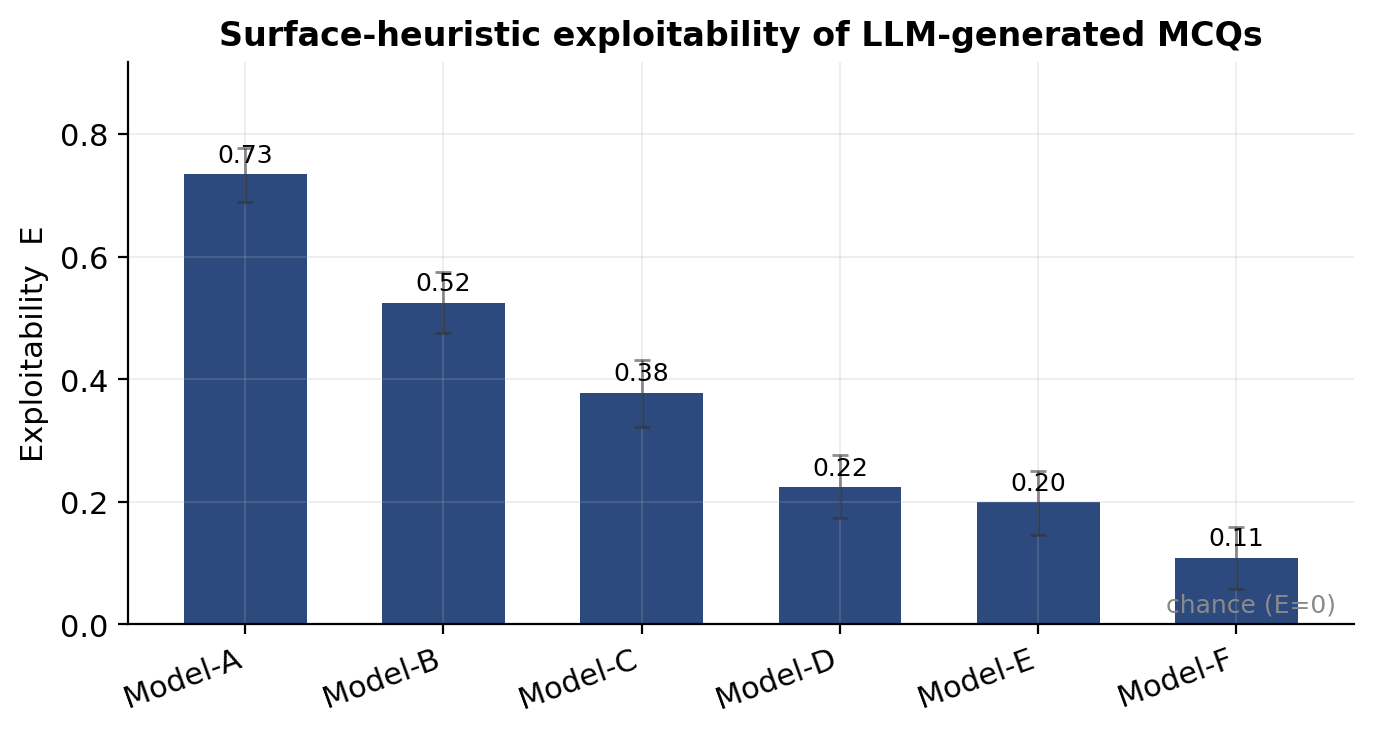
\includegraphics[width=\columnwidth]{fig_exploitability_by_model_synthetic.png}
\caption{Exploitability $E$ by generator on the synthetic corpus
(illustrative). Bars show the normalized above-chance advantage of an
always-longest strategy; whiskers are bootstrap 95\% CIs. The gradient is
injected ground truth that the metric recovers.}
\label{fig:expl}
\end{figure}

\begin{figure}[t]
\centering
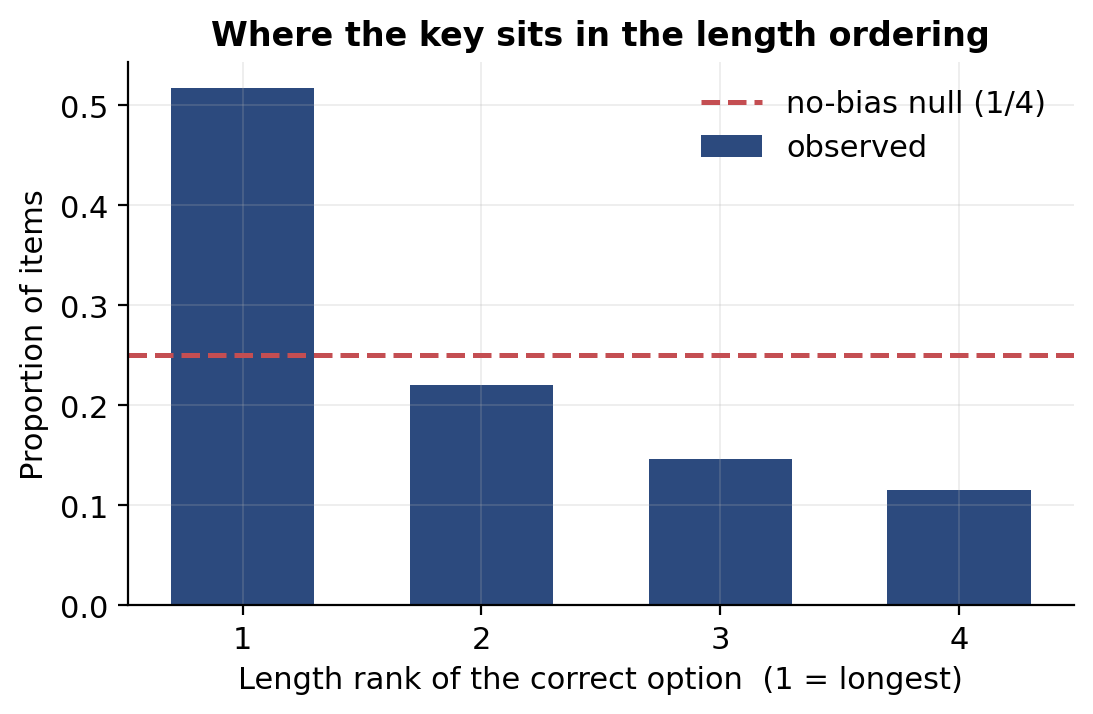
\includegraphics[width=\columnwidth]{fig_rank_distribution_synthetic.png}
\caption{Distribution of the correct option's length \emph{rank} (1 = longest)
on the synthetic corpus (illustrative). Under no leakage every rank would hold
$25\%$; the mass at rank~1 is the signature of answer-length leakage.}
\label{fig:rank}
\end{figure}

\subsection{Variation across subject and difficulty}
Figure~\ref{fig:heat} shows Exploitability across the subject\,$\times$\,
difficulty grid. Because the synthetic generator injects bias primarily as a
function of model strength, the grid is comparatively flat across cells; in a
real study this same heatmap is the instrument for detecting whether, for
example, ``hard'' items leak more (a plausible hypothesis if models over-qualify
difficult keys). We include it to demonstrate the per-cell estimator and its
visualization.

\begin{figure}[t]
\centering
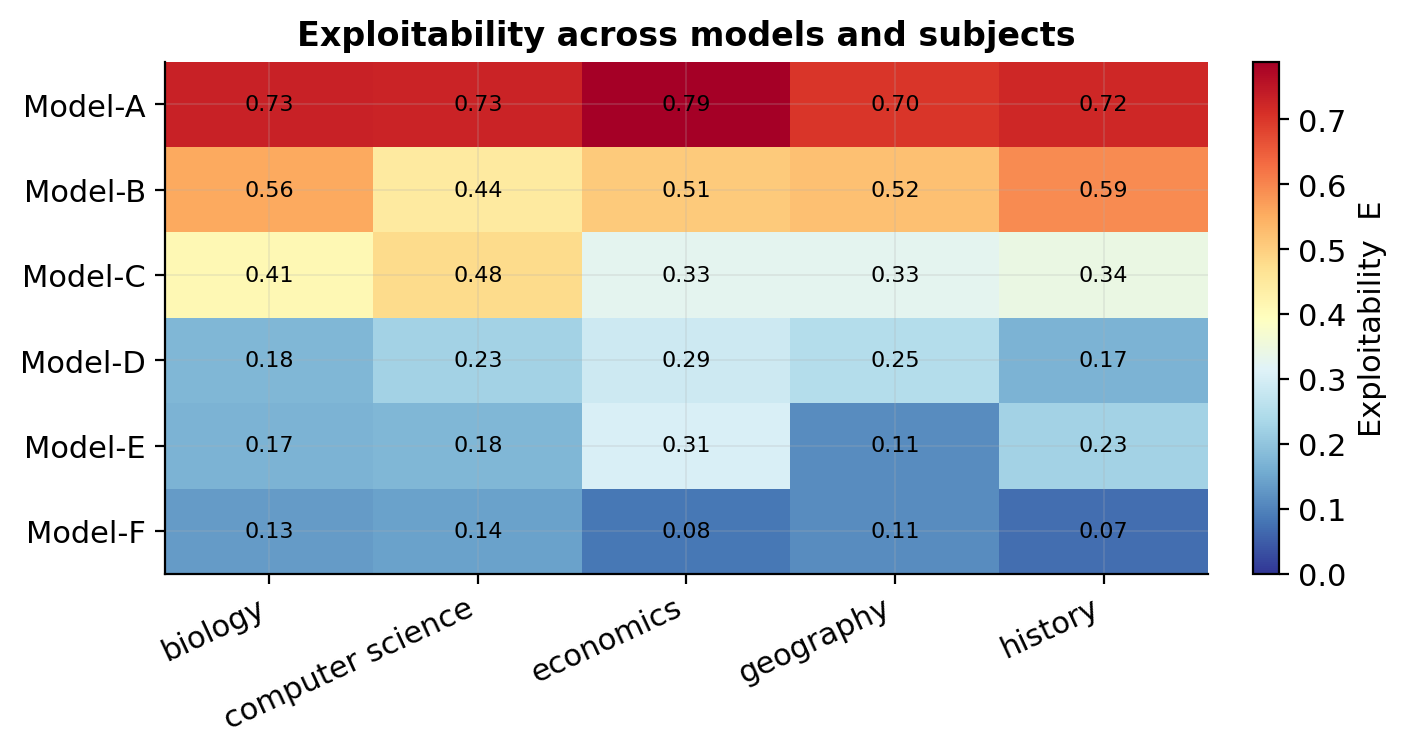
\includegraphics[width=\columnwidth]{fig_heatmap_synthetic.png}
\caption{Exploitability $E$ across subject\,$\times$\,difficulty on the
synthetic corpus (illustrative). The panel demonstrates the per-cell estimator
that a real study would use to localize where leakage concentrates.}
\label{fig:heat}
\end{figure}

\subsection{Mitigation: before vs.\ after}
We apply the hardening pipeline (Algorithm~\ref{alg:harden}) to the synthetic
corpus and recompute every metric. Table~\ref{tab:mitig} and
Figure~\ref{fig:mitig} summarize the effect. The fraction of items flagged
leaky falls from $71.4\%$ to $2.9\%$. Exploitability drops from $E={+}0.361$ to
$E={-}0.061$---statistically indistinguishable from, and slightly below,
chance---while the leakage AUC moves from $0.698$ to $0.439$ and the mean
differential from ${+}80.97$ to ${-}16.68$ characters. In other words, after
hardening, the longest option is no longer a reliable guess, and a length-only
classifier does no better than chance. The mitigation over-corrects $\bar\delta$
slightly negative; this is a tunable property of the deterministic matcher and
can be centered by adjusting the target band. These before/after numbers quantify
the \emph{length} signal only; they are not a measure of item quality, which we do
not evaluate here (\S\ref{sec:limitations}).

\begin{table}[t]
\centering
\caption{Mitigation before/after on the \textbf{synthetic} corpus
(illustrative). Lower magnitude is better for every row; the target for $E$,
AUC, and $\bar\delta$ is parity (0, 0.5, 0).}
\label{tab:mitig}
\small
\begin{tabular}{lrrr}
\toprule
Metric & Before & After & $\Delta$\\
\midrule
Longest-Answer Accuracy & 0.521 & 0.204 & -0.317\\
Exploitability $E$ & 0.361 & -0.061 & -0.422\\
Leakage AUC & 0.698 & 0.439 & -0.259\\
Mean differential $\bar\delta$ (chars) & 80.969 & -16.679 & -97.648\\
\bottomrule
\end{tabular}
\end{table}

\begin{figure}[t]
\centering
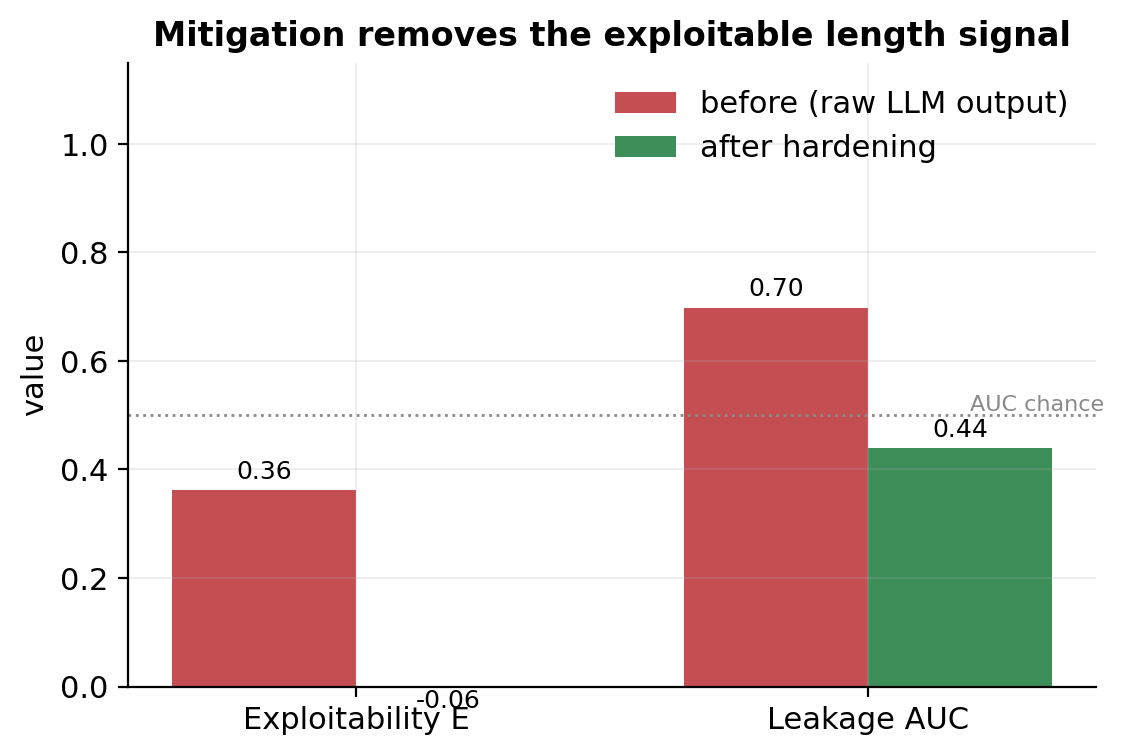
\includegraphics[width=\columnwidth]{fig_mitigation_synthetic.png}
\caption{Leakage metrics before and after hardening on the synthetic corpus
(illustrative). The auditing gate plus length-balancing drives exploitability
to parity and the length-only AUC to chance.}
\label{fig:mitig}
\end{figure}

\subsection{Distributional view}
Figure~\ref{fig:delta} shows the full distribution of the per-item verbosity
differential before and after mitigation. Pre-mitigation mass sits to the right
of zero (keys longer than distractors); post-mitigation the distribution
recenters near zero, consistent with the aggregate statistics above.

\begin{figure}[t]
\centering
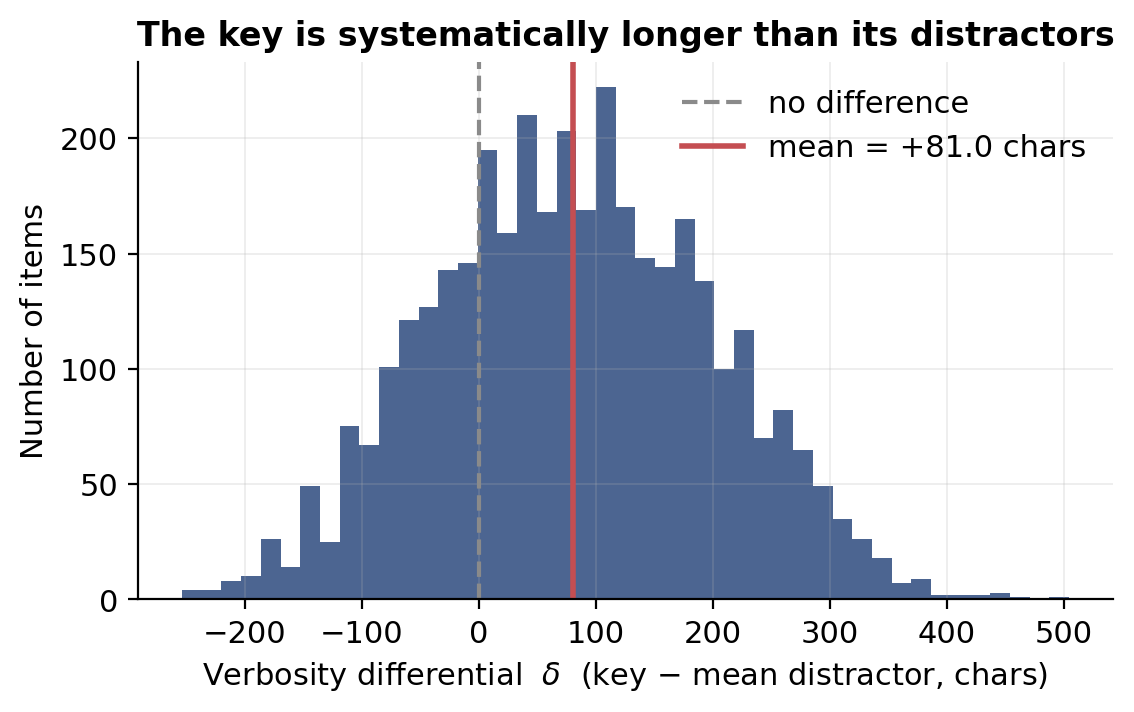
\includegraphics[width=\columnwidth]{fig_delta_distribution_synthetic.png}
\caption{Per-item verbosity differential $\delta$ (key minus mean distractor,
characters) before and after mitigation on the synthetic corpus (illustrative).
Recentering near zero indicates the length signal has been removed.}
\label{fig:delta}
\end{figure}

%==============================================================
\section{Discussion}
\label{sec:discussion}

\paragraph{Interpreting the synthetic results.} The pipeline does what it is
designed to do: the metrics recover injected bias with correct ordering and
calibrated magnitudes, the statistical tests behave, and the mitigations remove
the leak on controlled ground truth. This is necessary groundwork---an effect
this consequential should be measured with an instrument that has been
\emph{verified} end to end (software verification, not measurement validation)
before it is pointed at production systems. What the
synthetic study cannot tell us is the \emph{real} magnitude for Claude,
ChatGPT, Gemini, Grok, DeepSeek, or Perplexity; that requires running the
harness against the live endpoints (\S\ref{sec:future}).

\paragraph{Why a length signature is plausible in real models.} Three
non-exclusive mechanisms could produce keys that are systematically longer
than distractors. (1)~\emph{Qualification necessity}: a fully correct statement
often must include conditions and scope (``\,\dots under standard temperature
and pressure''), whereas a plausible-but-wrong option can be crisp; correctness
and length may be correlated for content reasons. (2)~\emph{Verbosity reward}:
alignment from human feedback can reward thoroughness, and judges prefer longer
answers \citep{zheng2023judging,saito2023verbosity}; a model may carry this
disposition into the option it is most committed to defending---the key.
(3)~\emph{Distractor-generation strategy}: models may generate distractors by
lightly perturbing or truncating the key, yielding shorter wrong options as a
by-product. These mechanisms are hypotheses; behavioral testing with the
harness can distinguish them (e.g., by checking whether the differential
persists when the model is asked to justify each option), but confirming
internal causes would require model-internal access we do not assume.

\paragraph{Connection to established theory.} Our metrics operationalize
construct-irrelevant variance \citep{messick1989validity}: $E>0$ is direct
evidence that a non-content feature predicts the key, and a ``pick-the-longest''
test-taker is exercising classical test-wiseness
\citep{millman1965testwiseness}. The novelty is not the existence of the flaw,
long known for human writers \citep{haladyna2002review,tarrant2006frequency},
but its potential systematicity under LLMs and the fact that it can be
\emph{audited and repaired automatically} at generation time.

\paragraph{Implications for practice.} The auditor (Algorithm~\ref{alg:audit})
is cheap enough to run on every machine-authored quiz and to embed in
authoring tools as a gate; it requires no model access, only the items. The
hardening step integrates with any LLM authoring loop. For institutions, the
form-level balancer offers a defense even when item-level differences are
small. For researchers, the metric suite provides a common yardstick so that
``which model leaks least'' becomes an answerable, reproducible question.

%==============================================================
\section{Conclusion}
\label{sec:conclusion}

We framed answer-length leakage in LLM-generated MCQs as a measurable threat to
assessment validity, defined a reusable exploitability-oriented metric suite
(LAA, $E$, $\bar\delta$, leakage AUC), built a provider-agnostic harness to
collect items under a length-neutral prompt, and delivered a generation-time
mitigation toolkit with a before/after protocol. On a clearly labeled synthetic
corpus the suite recovers injected bias and the toolkit drives exploitability
from $E={+}0.36$ to parity while cutting leaky items from $71\%$ to $3\%$.
Answering the research questions \emph{on the synthetic corpus}: leakage
\emph{is} definable and quantifiable (RQ1); the suite is sensitive enough to
resolve the injected model-level differences (RQ2); a longest-option strategy
beats chance on leaky corpora and length carries substantial information about the
key (RQ3); and lightweight mitigations drive the measured length signal to parity
without discarding items (RQ4). We did \emph{not} evaluate pedagogical item
quality, and the deterministic rewriter used in the demonstration manipulates
length only; whether a length-balancing rewrite preserves item quality is left to
future work (\S\ref{sec:future}). The contribution is a deployable measurement-
and-mitigation stack; the open empirical question---the magnitude in real
commercial systems---is one we have made \emph{straightforward to answer} with
the included harness and preregistered protocol.

%==============================================================
\section{Limitations}
\label{sec:limitations}

We are explicit about what this study does and does not establish.

\begin{itemize}[leftmargin=1.3em,itemsep=2pt,topsep=2pt]
\item \textbf{No real-model measurements.} Every number in
\S\ref{sec:results} comes from a synthetic corpus with injected bias. We do not
report, and the reader must not infer, the leakage of any named commercial
model. The synthetic study verifies the tooling only.
\item \textbf{The reported magnitudes are illustrative.} The headline reduction
($E:{+}0.36\!\to\!{-}0.06$) reflects controlled ground truth and tuned
thresholds; real corpora may differ in both baseline leakage and achievable
reduction.
\item \textbf{Length is a proxy.} Character/word length is one surface cue;
keys may also leak through specificity, grammaticality, or option position. We
measure length; we do not claim it is the only or dominant cue.
\item \textbf{Item quality is not evaluated.} We measure option-length
characteristics, not whether mitigated items remain valid, answerable, or
pedagogically sound. The deterministic rewriter used to produce the before/after
numbers neutralizes length by trimming or padding text and is \emph{not} a
meaning-preserving editor; a real LLM rewriter (\S\ref{sec:mitigation}) and an
explicit quality assessment (e.g.\ expert review, readability, answerability) are
prerequisites for any claim that mitigation preserves item quality.
\item \textbf{Prompt sensitivity.} Real measurements will depend on the
elicitation prompt, decoding temperature, and model version. Our length-neutral
prompt is one defensible choice; results may not transfer across prompts.
\item \textbf{Model drift.} Commercial models are updated frequently; any
real-world estimate is a snapshot and may not persist.
\item \textbf{Mechanism is hypothesized.} We offer behavioral hypotheses for
why keys might be longer; we do not have model-internal access and do not claim
to have identified the cause.
\item \textbf{No human-subject data yet.} We have not measured how much a real
``pick-the-longest'' strategy raises scores for real students; that is a
separate, IRB-governed study (\S\ref{sec:future}).
\end{itemize}

%==============================================================
\section{Future Work and Recommendations}
\label{sec:future}

\paragraph{Preregistered real-model study.} Run \texttt{src/collect.py} against
the six assistants with institutional API access, holding the grid
($5$ subjects $\times$ $3$ difficulties) and cell size fixed, with temperature
and model versions logged. Pre-register the primary hypothesis ($E>0$ overall),
the per-model comparison, and the subject/difficulty interaction. Estimate
sample size for a target CI half-width on $E$; the bootstrap machinery is
already in place.

\paragraph{Human-subject validation of exploitability.} With IRB approval and
informed consent, present students with leaky and hardened forms and measure
the score lift attributable to a longest-option strategy, and whether students
spontaneously discover it. This converts $E$ from a corpus statistic into a
measured integrity risk.

\paragraph{Mechanism probes.} Use the harness to test the qualification,
verbosity-reward, and distractor-strategy hypotheses behaviorally (e.g., ask
models to justify each option, or to generate distractors first), and study
whether instruction-level interventions reduce leakage at the source.

\paragraph{Beyond length.} Extend the metric suite to other construct-
irrelevant cues (option specificity, ``all/none of the above,'' grammatical
agreement, position) so that authoring tools can audit a battery of leaks, not
just one.

\paragraph{Deployment.} Package the auditor as a plug-in for common quiz and
LMS authoring flows so that every machine-generated item is screened by
default, turning the mitigation from a research artifact into infrastructure.

%==============================================================
\section*{Reproducibility and Artifacts}
\addcontentsline{toc}{section}{Reproducibility and Artifacts}
All metrics (\texttt{metrics.py}), the collection harness
(\texttt{collect.py}), the mitigation toolkit (\texttt{mitigate.py}), the
synthetic generator (\texttt{synthesize\_demo.py}), and the analysis driver
(\texttt{analyze.py}) are included, along with the synthetic corpus, the
generated tables, and all figures. The pipeline is deterministic given a seed.
See Appendix~\ref{app:repo} for the layout and commands.

%==============================================================
\section*{Ethical Considerations}
\addcontentsline{toc}{section}{Ethical Considerations}
This work aims to \emph{protect} assessment integrity. The metrics and harness
could in principle help a student exploit leaky quizzes; we mitigate this by
pairing every measurement tool with a remediation tool and by framing the
contribution around auditing and repair. Any human-subject component must
proceed under institutional review with informed consent and data
minimization. We report on synthetic data precisely to avoid publishing
unverified claims about named systems.

%==============================================================
\appendix
\section{Repository Layout and Commands}
\label{app:repo}
\small
\begin{verbatim}
llm-mcq-length-bias/
  src/metrics.py        # LAA, E, delta, AUC, logistic
  src/collect.py        # 6-provider harness (--dry-run)
  src/mitigate.py       # auditor + 3 mitigations
  src/synthesize_demo.py# synthetic corpus generator
  src/analyze.py        # driver: tables + figures
  data/                 # corpora (jsonl)
  results/              # results_*.json, *.tex tables
  figures/              # *.png/*.pdf
  paper/                # main.tex, references.bib
\end{verbatim}
Typical workflow:
\begin{verbatim}
# 1. validate pipeline offline (no keys)
python src/collect.py --dry-run --out data/dry.jsonl
python src/synthesize_demo.py --out data/synthetic_mcq.jsonl
python src/analyze.py --data data/synthetic_mcq.jsonl \
                      --tag synthetic
# 2. real run (needs your API keys, ToS-compliant);
#    run collect.py once per provider, then concatenate
export ANTHROPIC_API_KEY=...   # etc. per provider
python src/collect.py --provider anthropic --model <id> \
                      --out data/corpus_claude.jsonl
cat data/corpus_*.jsonl > data/real.jsonl
python src/analyze.py --data data/real.jsonl --tag real
\end{verbatim}

\section{Metric Summary}
\label{app:metrics}
\small
For a corpus with items $(s,\mathcal{O},k)$ and length $\ell(\cdot)$:
$\mathrm{LAA}$ is the longest-option score (Eq.~\ref{eq:laa});
$E=(\mathrm{LAA}-\bar c)/(1-\bar c)$ normalizes the above-chance advantage
(Eq.~\ref{eq:expl}); $\bar\delta$ is the mean key$-$distractor differential
(Eq.~\ref{eq:delta}); the leakage AUC is the key-outranks-distractor
probability (Eq.~\ref{eq:auc}); and the logistic odds ratio per SD expresses
leakage as a single multiplier. All are reported with bootstrap CIs and
per-group breakdowns.

\balance
\bibliographystyle{unsrtnat}
\bibliography{references}

\end{document}
